% !TeX root = ../sustechthesis-example.tex

\chapter{如何构建RL控制训练模型}
在这部分将阐述关于如何使用强化学习来进行运动控制的内容。相比于传统的基于模型的控制方法,该方法通过在模拟环境中训练控制策略,可以更好地适应复杂的非线性系统动力学和环境不确定性,并且能够实时响应用户命令和环境变化。在这里我们主要关注如何使用强化学习来训练机械狗类型的足式和轮式机器人控制器。


\section{强化学习控制}

本部分内容的探究起点是这篇文献的内容:\emph{Control of Wheeled-Legged Quadrupeds Using Deep Reinforcement Learning}\cite{Lee_Bjelonic_Hutter_2023}


\subsection{强化学习的基本概念}

在强化学习中,控制问题被建模为一个马尔可夫决策过程(Markov Decision Process)。MDP是一个RL中常用的用于随机控制过程建模的数学框架,它定义了一个包含状态空间、动作空间、奖励函数和状态转移函数的元组,描述了一个决策过程的基本组成部分。在MDP中,每个时间步骤代理从周围环境中观察到某个状态$s_t \in \mathcal{S}$,并输出一个动作$a_t \in \mathcal{A}$,接着环境通过状态转移函数$p(s_{t+1}|s_t, a_t)$演化到新的状态$s_{t+1}$,并且根据奖励函数给出相应的奖励$r_t\in \mathcal{R}:\mathcal{A}\times\mathcal{S}\to \mathbb{R}$和对更新后的环境状态的观察结果作为下一周期的$s_t$。
代理可以根据$\theta$参数化的随机策略$\pi_\theta(a_t|s_t)$来采取行动。RL通过与环境交互来更新参数$\theta$以最大化累计折扣奖励(cumulative discounted rewards)$\mathbb{E} [\sum_{t=k}^{\infty}\gamma^t r_t]$,其中$k$是当前时间步长(timestep),$\gamma$是折扣因子(discount factor)。

\subsection{如何实现基于深度强化学习的控制器在时间环境中的部署和优化}

\begin{enumerate}
    \item 在仿真环境中训练控制器:使用深度强化学习算法在仿真环境中训练控制器,使其能够完成所需的任务。在训练过程中,可以使用特权训练方法来提高训练效率和性能。
    \item 部署控制器到实际环境中:将训练好的控制器部署到实际环境中,例如机器人或移动设备。在实际环境中,控制器将接收传感器数据并输出动作命令。
    \item 优化控制器:在实际环境中,可以使用在线学习方法来进一步优化控制器的性能。例如,可以使用模型预测控制方法来对控制器进行在线微调。
\end{enumerate}

需要注意的是,在实际环境中,传感器数据可能会受到噪声和不确定性的影响,因此需要设计鲁棒性强的控制器来应对这些问题。此外,还需要考虑实际环境中的安全性和可靠性问题。


\section{RL的构建、训练和部署}
\subsection{MDP的制定}

一个MDP是由一个元组定义,它包含状态空间$\mathcal{S}$、动作空间$\mathcal{A}$、奖励函数$r_t(s_t|s_{t+1})$、转移函数$p(s_{t+1}|s_t, a_t)$。这套定义方式和文献类似\cite[p]{Miki_Lee_Hwangbo_Wellhausen_Koltun_Hutter_2022}。
这个策略的环境观察部分包括周围地面的高度扫描结果、来自IMU的本体姿态信息、来自各个关节点的编码器信息。
运动被定义为一个21维的向量,包括步态参数偏移、关节点位置偏移和轮子速度控制指令。
奖励函数由表\ref{table:reward_functions}定义。
\begin{table}[h!]
    \begin{center}
      \caption{Reward functions. (The velocities are defined in the base frame)}
      \label{table:reward_functions}
      \begin{tabular}{l|l} % <-- Alignments: 1st column left, 2nd middle and 3rd right, with vertical lines in between
        \hline
        \multicolumn{2}{l}{\textbf{Reward terms}}\\
        \hline
        Linear velocity & $1.5 \exp(-3(v^{xy}-\hat v^{xy})^2)$\\
        Angular velocity & $1.0\exp(-3(\omega^z-\hat\omega^z)^2)$\\
        Base motion penalty & $0.8\exp(-(v^z)^2)+\exp(-(\omega^{x,y})^2)$\\
        Torque penalty & $-10^{-6} \|\tau\|^2$\\
        Joint speed penalty & $-0.05\sum_{i=0}^{12}\max(|\dot \phi_i|-\dot\phi_{jslim},0)^2$\\
        Action smoothness penalty & $-0.05|a_{t-2}-2a_{t-1}+a_t|$\\
        \hline
        \multicolumn{2}{l}{\textbf{Symbols}}\\
        \hline
        $\dot \phi_{jslim}$ & Maximum joint speed\\
        $\tau$ & Vector of joint torques\\
        $f_c$ & Foot contact state\\
        $\hat{(\cdot)}$ & Traget quantity\\
        $(\cdot)_g$ & Sub-goal quantity\\
        $\mathbb{1}_{(condition)}(\cdot)$ & Indicator function\\
        \hline
      \end{tabular}
    \end{center}
\end{table}

状态转换遵循刚性的动力学模拟,当机器人主体接触地面或到达关节扭矩和速度限制时,该训练集终止。

\subsection{RL模型的训练方式}

我们遵循Lee等人\cite{Lee_Hwangbo_Wellhausen_Koltun_Hutter_2020}的特权训练方法。我们首先使用on-policy RL算法\cite{Schulman_Wolski_Dhariwal_Radford_Klimov_2017}训练具有无噪声模拟状态(特权信息)的教师策略。换句话说,我们用额外的模拟状态附加给$s_t$,包括地面摩擦系数、地面反作用力以及每个连杆的接触状态。特权信息使教师策略能够学习地形自适应行为。由于无噪声和准确的模拟状态,教师策略快速收敛到高性能策略。在桌面PC上使用PPO算法\cite{Schulman_Wolski_Dhariwal_Radford_Klimov_2017},教师策略训练大约需要8小时。然后我们为实际部署训练一个学生策略。学生策略在没有特权信息和观察噪声的情况下模仿老师。通过模仿学习\cite{Ross_Gordon_Bagnell_2010},它学习从嘈杂的真实世界观察序列构建世界的内部表示。以这种方式训练的策略已被证明在具有高干扰和噪声观测的真实世界环境中更具适应性和鲁棒性\cite{Lee_Hwangbo_Wellhausen_Koltun_Hutter_2020}。

\subsection{训练平台和部署}

训练采用的平台有Raisim\cite{Hwangbo_Lee_Hutter_2018, Lee_Bjelonic_Hutter_2023}仿真器、英伟达的Isaac\cite{Rudin_Hoeller_Reist_Hutter_2021}仿真器。

\begin{note}
    2023-10-06 18:19:57,感觉强化学习者部署起来也不是件容易得事情呀。后面关于运动控制建模的方式就先不看了。重点关注用强化学习做控制要关注的内容。
\end{note}


\section[RL的实现和部署2]{RL的实现和部署2\cite[p10-12]{Miki_Lee_Hwangbo_Wellhausen_Koltun_Hutter_2022}}


\begin{figure}
  \centering
  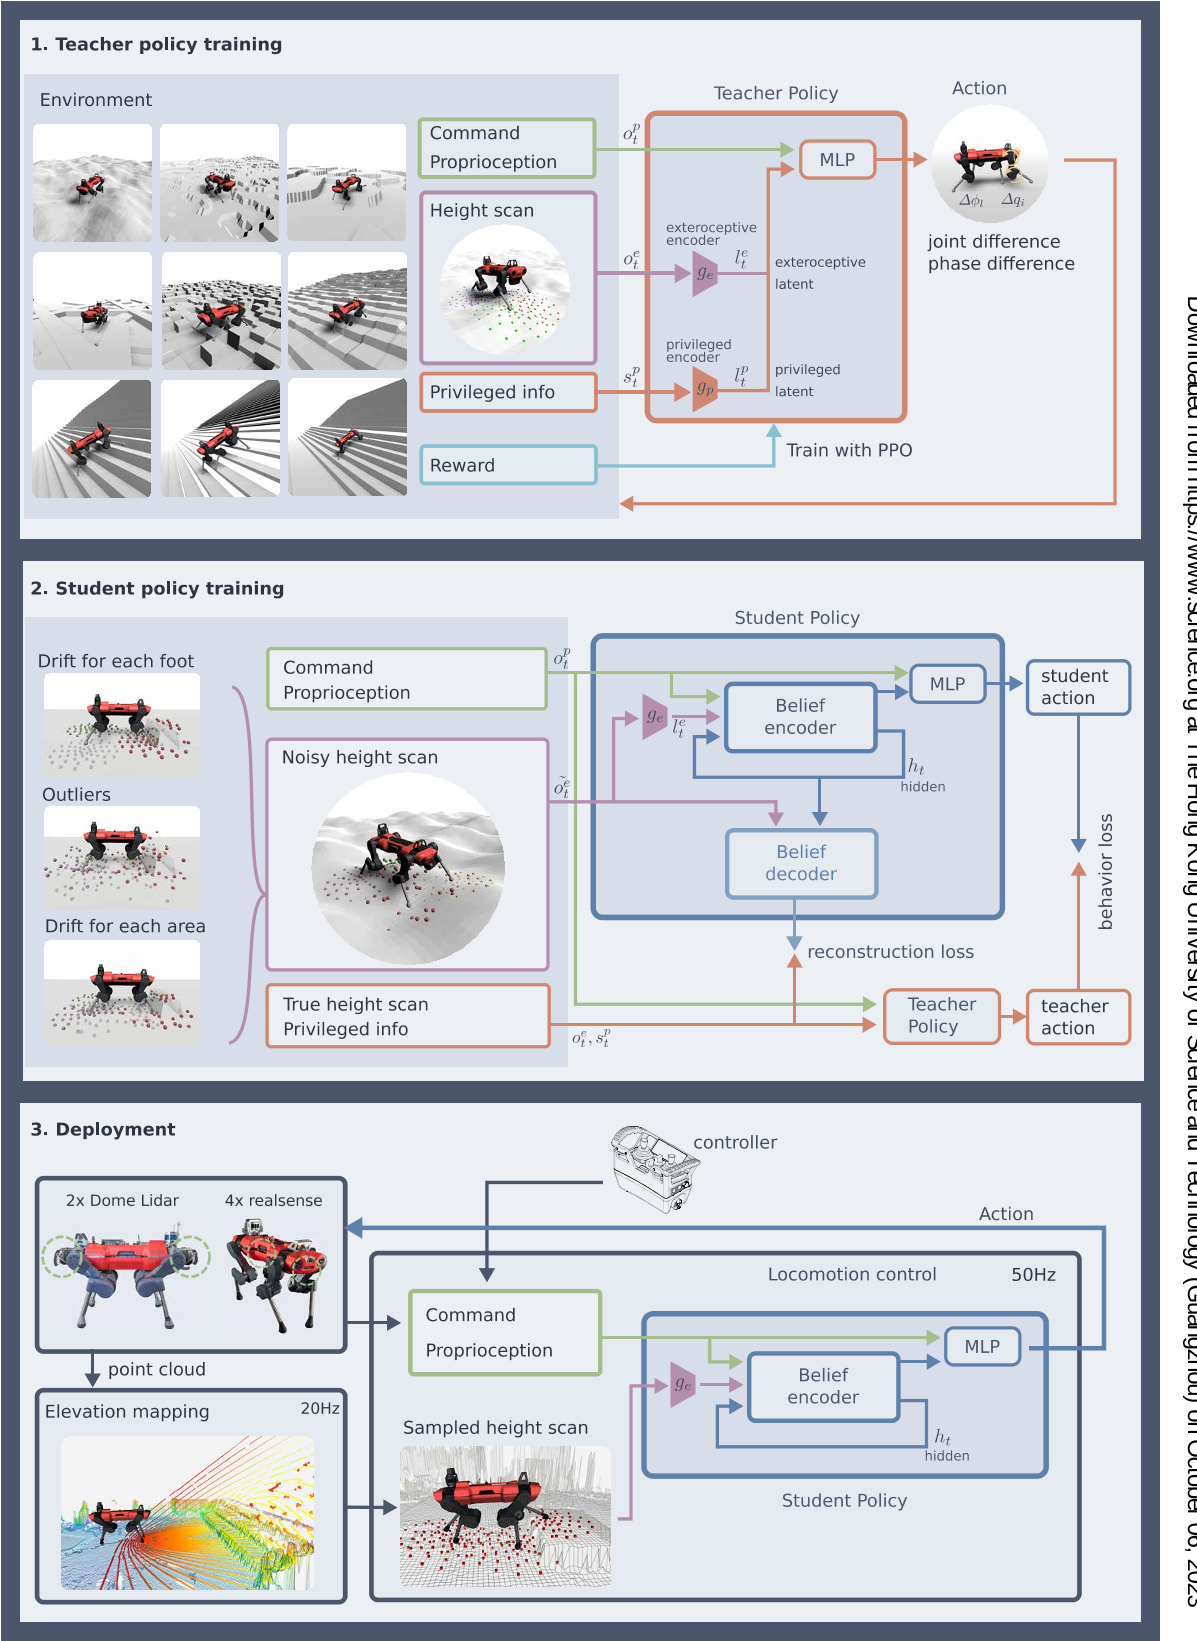
\includegraphics[width=1.0\linewidth]{train_process.png}
  \caption{RL implementation process\cite[p9]{Miki_Lee_Hwangbo_Wellhausen_Koltun_Hutter_2022}.}
  \label{fig:process}
\end{figure}

% \textcolor{gray}{\small 这节主要参考文献\cite[p10-12]{Miki_Lee_Hwangbo_Wellhausen_Koltun_Hutter_2022}。}

整个神经网络的训练是在仿真环境中完成的,然后采用\emph{zero-shot sim-to-real}的转换部署到实际的额机器人上。整个方法分为三个阶段,如图\ref{fig:process}所示。
\begin{enumerate}
  \item 首先,使用RL训练教师策略,以在随机生成的具有随机干扰的地形上遵循随机目标速度。该策略可以访问特权信息,例如无噪声地形测量、地面摩擦和引入的扰动。
  \item 在第二阶段,训练学生策略重现教师策略的动作,而不使用这种特权信息。学生策略构造一个信念状态来使用循环编码器捕获未观察到的信息,并根据该信念状态输出一个动作。在训练期间,我们利用两个损失:\emph{行为克隆损失}和\emph{重建损失}。行为克隆损失旨在模仿教师策略。重新构造损失鼓励编码器产生信息丰富的内部表示。
  \item 最后,我们将学习到的学生策略转移到物理机器人上,并将其与机载传感器在现实世界中部署。机器人通过整合来自板传感器的深度数据和从构建的高程图中采样高度读数来构建高程图,以形成策略的外部感知输入。这种外部感知输入与本体感觉数据相结合,并提供给神经网络,该网络产生执行器命令。\emph{板上传感器和自身构建等高图融合}
\end{enumerate}

\subsection[问题描述]{问题描述}

我们在离散时间动力学中制定了我们的控制问题,其中环境完全由时间步$t$的状态$s_t$定义。该策略实施一个动作$a_t$并且从环境中获得一个观测结果$o_t$,这个测量结果来自观测模型$\mathcal{O}(o_t|s_t,a_t)$。接着环境以$P(s_{t+1}|s_t, a_t)$的概率转移到下一个状态$s_{t+1}$并给出一个奖励$r_{t+1}$。

当所有状态都可以被观测的实况下,也即$o_t=s_t$时,整个问题可以被看做一个马尔可夫决策过程\emph{Markov decision process(MDP)}。然而,当存在不可观察性的信息时,例如外力或完整的地形信息,动力学被建模为部分可观察的马尔可夫决策过程\emph{partially observable Markov decision process(POMDP)}。

RL的目标是找到一个能够使得未来轨迹的预期折扣奖励最大化的策略$\mathbfit{\pi}^*$,以使得:
\begin{align}
  \mathbfit{\pi}^*=\underset{a}{argmax}E[\sum_{t=0}^{\infty}\gamma^t r_t]
\end{align}

已经开发了许多RL算法来解决完全可观察的MDP问题,并且易于用于训练。然而,POMDP问题的情况更具挑战性,因为状态不能完全观察到。这通常通过从历史的观察结果$o_0, \cdots, o_t$中构建一个信念状态$b_t$\emph{belief state}以尝试构建完全状态的方式来解决。在深度RL中,这通常是通过堆叠一系列先前的观察结果\cite[p]{Mnih_Kavukcuoglu_Silver_Graves_Antonoglou_Wierstra_Riedmiller_2013}或使用可以压缩过去信息的架构来完成的,例如循环神经网络 (RNN) \cite[p]{Zhu_Li_Poupart_Miao_2017}或时间卷积网络\cite[p]{Lee_Hwangbo_Wellhausen_Koltun_Hutter_2020,Bai_Kolter_Koltun_2018}。

从头开始训练一个天真地处理序列数据的复杂的神经网络策略可能很耗时\cite[p]{Lee_Hwangbo_Wellhausen_Koltun_Hutter_2020}。因此,我们使用特权学习(45),我们首先训练一个具有特权信息的教师策略,然后通过监督学习将教师策略提炼为学生策略\cite[p]{Chen_Zhou_Koltun_Krähenbühl_2019}。

\begin{enumerate}
  \item 训练环境:
  \item 地形:
  \item 域随机化:
  \item 片段终止条件:
\end{enumerate}

\subsection[教师策略训练]{教师策略训练}

在训练的第一阶段,我们的目标是找到一个可以访问完美、特权信息的最佳参考控制策略,并使ANYmal在随机生成的地形上遵循所需的命令速度。命令需求随机生成并构成一个向量$\mathbfit{v}_des\in \mathbb{R}^3=(v_x,v_y,w)$,其中$v_x, v_y$分别表示在机器人自身坐标系下的纵向速度和横向速度,$w$表示自转速度。

我们采用近端策略优化\emph{proximal policy optimization(PPO)}\cite[p]{Schulman_Wolski_Dhariwal_Radford_Klimov_2017}来训练教师策略。教师策略被建模为一个高斯策略,$a_t~\mathcal{N}(\pi_{\theta}(o_t=s_t),\sigma I)$,其中$\pi_{\theta}$由用$\theta$参数化的多层感知器\emph{multilayer perceptron(MLP)}实现,$\sigma$表示每个动作之间的方差。

\subsection[观测和行动]{观测和行动}

教师策略的观察定义为$o_t^{teacher}=(o_t^p, o_t^e, s_t^p)$,其中$o_t^p$表示本体感觉观察\emph{proprioception observation},$s_t^e$表示外部观察\emph{exteroceptive observation},$s_t^p$表示特权状态\emph{privileged state}。
\begin{itemize}
  \item $o_t^p$包含本体速度、转动、节点位置和速度历史、动作历史、每条腿的相位;
  \item $o_t^e$是每只脚周围高度样本的向量,包括五种不同的半径;
  \item $s_t^p$包括接触状态、接触力、接触法线、摩擦系数、大腿和小腿接触状态、施加到身体上外部力和力矩、摆动阶段持续时间;
\end{itemize}

我们的动作空间受到中心模式生成器的启发\cite[p]{Lee_Hwangbo_Wellhausen_Koltun_Hutter_2020}。每条腿$l={1,2,3,4}$保存一个相位变量$\phi_l$并定义了基于相位的标称轨迹。这个标称轨迹是一个脚尖的步进运动,我们使用逆运动学来计算每个关节执行器$i={1, \dots, 12}$的标称关节目标$q_i(\phi_l)$。来自策略的动作是相差$\Delta \phi_l$和关节位置目标残差$\Delta q_i$。\textcolor{gray}{\small 更详细相关内容看相关附件的S5。}

\subsection[策略构架]{策略构架}

我们将教师策略$\pi_{\theta}$建模为一个MLP。它包括三个MLP组成部分:外部感知编码器、特权编码器、主网络,如图\ref{fig:process}所示。
\begin{enumerate}
  \item 外部感知编码器$g_e$接收来自$o_t^e$的信息,然后输出一个小些的潜在表示$$l_t^e=g_e(o_t^e)$$
  \item 特权编码器$g_p$接收来自特权状态$s_t^p$的信息,然后输出一个潜在表示$$l_t^{priv}=g_p(s_t^p)$$
  \item 
\end{enumerate}

这些编码器将每个输入压缩为更紧凑的表示,并使得学生策略能更方便地重用一些教师策略组件。\textcolor{gray}{\small 更详细相关内容看相关附件的S6。}

\subsection[奖励函数]{奖励函数}

针对速度控制命令的跟随,我们定义正奖励;针对违反约束的情况,我们定义负奖励。指令跟随奖励定义如下:
\begin{align}
  \mathbfit{r}_{command}=\begin{cases}
    1.0, &if \mathbfit{v}_{des}\cdot\mathbfit{v}>|\mathbfit{v}_{des}|\\
    \exp(-(\mathbfit{v}_{des}\cdot\mathbfit{v})^2), &otherwise
  \end{cases}
\end{align}

其中$\mathbfit{v}_{des}\in\mathbb{R}^2$是所需的水平速度,$\mathbfit{v}\in\mathbb{R}^2$是身体坐标系下当前身体速度。同样的奖励机制也被应用与转动速度情况。

我们惩罚与期望速度正交的速度分量以及横摇、俯仰和偏航周围的身体速度。此外,我们使用整形奖励进行身体方向、关节扭矩、关节速度、关节加速度和脚滑以及小腿和膝盖碰撞。身体方向奖励用于避免身体的奇怪姿势。联合相关奖励术语用于避免过于激进的运动。脚滑和碰撞奖励术语用于避免它们。我们通过在模拟中查看策略的行为来调整奖励术语。除了遍历性能外,我们还检查了运动的平滑度。
\textcolor{gray}{\small 更详细相关内容看相关附件的S7。}

\subsection[课程]{课程}
随着策略性能的提高,我们使用两个课程来提高难度。
一个课程使用自适应方法\cite[p]{Lee_Hwangbo_Wellhausen_Koltun_Hutter_2020}调整地形难度,另一个改变元素,如奖励或使用逻辑函数\cite[p]{Hwangbo_Lee_Dosovitskiy_Bellicoso_Tsounis_Koltun_Hutter_2019}应用干扰。

对于地形课程,粒子滤波更新地形参数,使它们仍然具有挑战性,但在策略训练期间的任何时候都可以实现\cite[p]{Lee_Hwangbo_Wellhausen_Koltun_Hutter_2020}。

第二个课程将域随机化的幅度和一些奖励项(关节速度、关节加速度、方向、滑移和大腿和小腿接触)乘以单调递增且渐近趋势为 1 的因子:$$c_{k+1}=(c_k)^d$$

其中$c_k$是第$k$次迭代的课程因子,$d\in(0,1)$是收敛率。

\subsection[学生策略训练]{学生策略训练}

在我们训练好一个可以在特权信息的帮助下穿越各种地形教师策略后,我们就可以将其提炼成一个学生策略,该策略只能访问真实robot上可用的信息。我们使用与教师策略相同的训练环境,但在学生高度样本观察中添加额外的噪声:$o_t^{student}=(o_t^p,n(o_t^e))$,其中$n(o_t^e)$是一个用于高度样本输入的噪声模型。该噪声模型模拟了现场部署过程中经常遇到的外部感觉的不同失败案例,具体如下。

当外部感觉中存在较大的噪声时,它变得不可观察;因此,动力学被认为是POMDP。此外,由于缺乏直接测量的传感器,特权状态是不可观察的。因此,该策略需要考虑顺序相关性来估计不可观察的状态。我们建议使用\emph{循环信念状态编码器}来组合外部感知和本体感觉的序列,以估计不可观察的状态作为信念状态。

学生策略由循环信念状态编码器和MLP组成,如图\ref{fig:process}所示。我们用$h_t$表示循环网络的隐藏状态。信念状态编码器接收$o_t^{sutdent},h_t$并输出一个潜在向量$b_t$,它表示信念状态。我们的目标是将信念状态$b_t$与编码所有运动相关信息的教师策略的特征向量($l_t^e, l_t^{priv}$)进行匹配。
接下来我们将$o_t^p$和$b_t$传入MLP,由它计算出最终的动作。MLP结构与教师策略相同,这样我们就可以重用教师策略的学习权重来初始化学生网络并加快训练速度。

学生策略的训练通过最小化两个损失以有监督的方式进行训练:行为克隆损失\emph{behavior cloning loss}和重建损失\emph{reconstruction loss}。
\begin{itemize}
  \item 克隆损失定义为给定相同状态和指令的学生动作和教师动作之间的平方距离。
  \item 重建损失定义为无噪声高度样本和特权信息($o_t^e, s_t^p$)及其与信念状态$b_t$的重建之间的平方距离。
\end{itemize}

我们通过推出学生策略来生成样本,以提高鲁棒性\cite[p]{Ross_Gordon_Bagnell_2010,Czarnecki_Pascanu_Osindero_Jayakumar_Swirszcz_Jaderberg_2019}。

\subsection[高度采样随机化]{高度采样随机化}

\begin{figure}
  \centering
  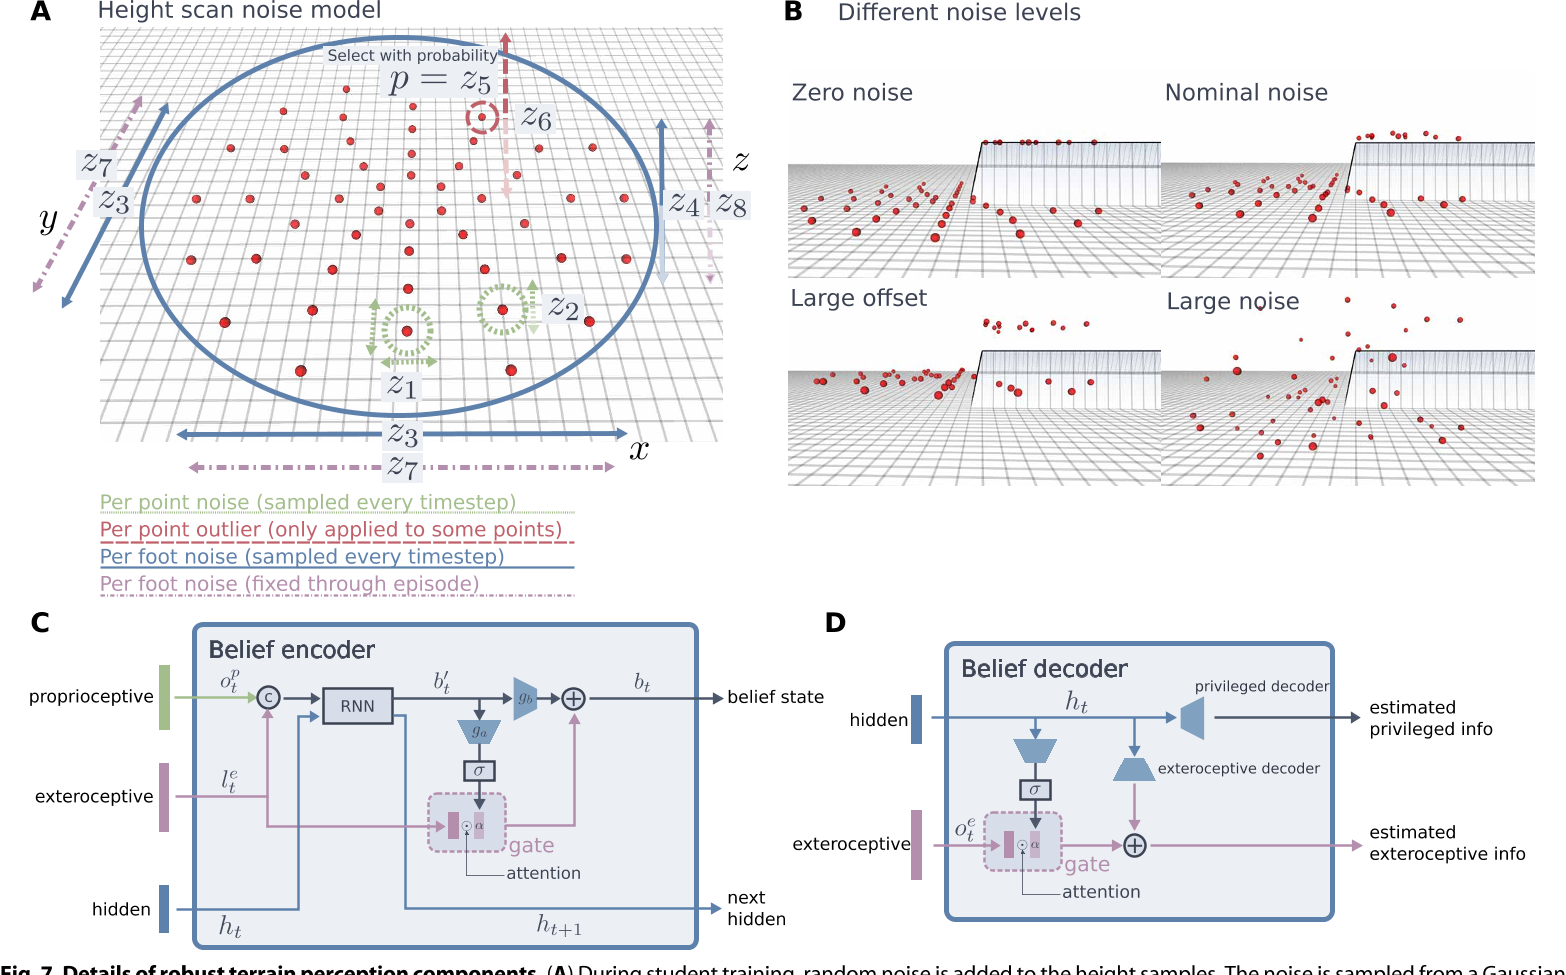
\includegraphics[width=1.0\linewidth]{terrain_perception.png}
  \caption{Robust terrain perception\cite[p10]{Miki_Lee_Hwangbo_Wellhausen_Koltun_Hutter_2022}.}
  \label{fig:terrain_perception}
\end{figure}

在学生训练过程中,我们使用参数化噪声模型$n(\sigma_t^e|o_t^e,z),z\in \mathbb{R}^{8\times 4}$将随机噪声注入到高度样本中。
我们在对高度进行采样时应用了两种不同类型的测量噪声,如图\ref{fig:terrain_perception}A所示:
\begin{enumerate}
  \item 横向移动扫描点。
  \item 扰动高度值。
\end{enumerate}

每个噪声值都是从高斯分布中采样的,噪声参数$z$定义方差。这两种类型的噪声都应用于三个不同的范围,所有这些都有自己的噪声方差:每个扫描点、每只脚和每一集。每个扫描点和每只脚的噪声值在每个时间步重新采样,而所有扫描点的表观轮廓噪声保持不变。

此外,我们定义了三个具有相关噪声参数$z$的映射条件来模拟不断变化的地图质量和误差源,如图\ref{fig:terrain_perception}B所示。
\begin{enumerate}
  \item 名义噪声假设常规操作期间具有良好的地图质量。
  \item 大偏移量噪声来模拟由于姿态估计漂移或可变形地形造成的地图偏移。
  \item 幅度较大的噪声来模拟由于遮挡或映射失败导致完全缺乏地形信息的情况。
\end{enumerate}

这三个映射条件在每个训练集的开头以60、30和10\%的比例选择。

最后,我们将每个训练地形划分为单元格,并向高度样本添加附加偏移量,具体取决于它采样的单元格。这模拟了不同地形特征的区域之间的转换,如植被和深度雪。参数向量$z$也是学习课程的一部分,其幅度随训练持续时间线性增加。

\textcolor{gray}{\small 更详细相关内容看相关附件的S8。}

\subsection[信念状态寄存器]{信念状态寄存器}

循环信念状态编码器编码不能直接观察到的状态。为了整合本体感受和外感受数据,我们引入了一个门控编码器,如图 7C 所示,灵感来自门控 RNN 模型\cite[p]{Cho_van_Merrienboer_Gulcehre_Bahdanau_Bougares_Schwenk_Bengio_2014,Hochreiter_Schmidhuber_1997}和多模态信息融合 (4-66)。

信念状态编码器学习使用一个可变的门控因子来控制外部感知信息通过的量。首先,内部感知$s_t^p$、从含噪声观测提取的外部感知$l_t^e=g_e(\widetilde o_t^e)$以及隐藏状态$s_t$被RNN模型编码成为一个中间信念状态$b_t{t'}$。它控制最终进入$b_t$的外部感知信息量:
\begin{align}
  b_{t'},h_{t+1}=RNN(o_t^p,l_t^e,h_t)\\
  \alpha = \sigma (g_a(b_{t'}))\\
  b_t = g_b(b_{t'})+l_t^e \odot \alpha
\end{align}

这里$g_a,g_b$是全连接的神经网络,$\sigma(\cdot)$是sigmoid函数。

解码器使用相同的门,用于重建特权信息和高度样本(图 7D)。这用于计算重建损失,它鼓励信念状态捕获有关环境的真实信息。我们使用 GR\cite[p]{Cho_van_Merrienboer_Gulcehre_Bahdanau_Bougares_Schwenk_Bengio_2014}作为我们的 RNN 架构。

\textcolor{gray}{门结构有效性的评估见第 S9 节。}

\subsection[部署]{部署}

我们在 PyTorch\cite[p]{Paszke_Gross_Massa_Lerer_Bradbury_Chanan_Killeen_Lin_Gimelshein_Antiga_et_al_2019}中训练策略,并在没有任何微调的情况下部署在机器人 zero-shot上。我们通过估计机器人的姿态,并相应地从传感器中调节点云读数,构建了一个以机器人为中心的2.5D高程图刷新率为20赫兹。该策略以50Hz运行,并从最新的高程图中映射采样高度;如果查询位置没有可用的地图信息,则填充随机采样的值。

我们开发了一个高程映射管道,用于在图形处理单元上快速地形映射,以并行化点云处理。我们遵循与Fankhauser等人\cite[p]{Fankhauser_Bloesch_Hutter_2018}使用的类似方法,以卡尔曼滤波的方式更新地图,另外按漂移补偿\emph{drift compensation}和光线投射\emph{ray casting}以获得更吻合的地图。这种快速映射实现对于保持快速处理速率和跟上我们的控制器实现的快速运动速度至关重要。

